\chapter{结果分析与相变模型}
	本章对温度反演结果进行深入分析，讨论各误差来源的贡献及改进方向，并基于准一维相变模型预测CO$_2$团簇成核位置与生长特征。
	\subsection{温度反演结果讨论}
	由第五章表\ref{tab:temp_result}可知，射流中心温度268~K，径向向外单调递增至305~K。这一趋势与欠膨胀射流的物理图像一致：射流核心区域因快速膨胀而温度最低，向外逐渐与环境空气混合，温度逐步回升。径向温度梯度在$R=0$--2~mm范围内较大（约6~K/mm），在$R=2$--5~mm范围内趋于平缓（约3~K/mm），反映了射流核心区与混合过渡区的不同热力学特性。
	温度分布与Fluent仿真结果（中心262~K）的偏差为2.3\%，在实验不确定度范围内（$\pm6$~K），证明了实验方法的可靠性。偏差可能来源于：
	\begin{itemize}
		\item 仿真采用理想气体模型，未考虑真实气体效应；
		\item 实验测量的空间分辨率（0.3~mm光斑）有限，无法完全分辨激波处的温度突变；
		\item Fluent网格分辨率及湍流模型引入的数值误差。
	\end{itemize}
	\subsection{误差来源分析}
	温度反演不确定度的主要贡献者依次为：
	\begin{enumerate}[label=(\arabic*)]
		\item \textbf{积分吸光度计算误差}（约$\pm4$~K）：来源于基线拟合的不确定性，在弱吸收区域（$R\ge4$~mm）尤为显著。改进方向包括采用更稳健的基线拟合算法（如多项式拟合阶数优化、Voigt线型约束拟合）和通过增加扫描周期数提升信噪比。
		\item \textbf{探测噪声}（约$\pm3$~K）：来源于探测器热噪声和电路噪声。后续可通过FPGA硬件累加平均进一步提升SNR。
		\item \textbf{光谱标定误差}（约$\pm2$~K）：来源于FSR峰位检测算法的精度限制。当前偏移约0.01-0.02~cm$^{-1}$，需改进峰值检测算法（如采用高斯拟合定心代替简单寻峰）。
		\item \textbf{HITRAN谱线参数不确定性}（约$\pm1$~K）：数据库中线强和低态能量的标定误差，属于系统误差，难以通过实验手段消除，但影响较小。
	\end{enumerate}
	综合以上分析，后续工作中应优先改进FSR标定精度和提升弱信号区域的信噪比，以进一步降低温度反演不确定度。
	\subsection{相变模型方法}
	基于Wu等（2021）的准一维相变模型代码，根据本实验条件（进口压力5~bar，小孔喷嘴，收缩角0$^\circ$，扩张角5$^\circ$）修改输入参数。模型耦合经典成核理论（CNT）与可压缩流动方程，核心方程：
	临界半径：
	\begin{equation}
		r^*=\frac{2\sigma}{\rho_l RT\ln S}
		\label{eq:rcrit}
	\end{equation}
	其中$\sigma$为表面张力，$\rho_l$为液相密度，$S=P_v/P_{\rm sat}$为过饱和度。
	成核速率：
	\begin{equation}
		J=\sqrt{\frac{2\sigma}{\pi m}}\frac{N_A}{\rho_l}
		\left(\frac{P_v}{kT}\right)^2
		\exp\left(-\frac{16\pi\sigma^3}{3\rho_l^2(RT)^3(\ln S)^2}\right)
		\label{eq:nucl_rate}
	\end{equation}
	液滴生长速率由扩散控制。模型沿流动方向迭代求解，判定凝结起始点（过冷度达到5~K时）。
	尝试了不同喉部面积（0.1~cm$^2$和0.01~cm$^2$）的模拟：喉部面积0.1~cm$^2$时模型可正常运行并输出结果；改为更接近实际的0.01~cm$^2$时计算发散，无法收敛。初步判断需调整网格密度、松弛因子或数值格式，后续将在模型中逐步加入非定常项以改善收敛性。
	\subsection{相变模型初步预测}
	基于Wu等（2021）的准一维相变模型代码，本节给出根据本实验条件修改后的模型计算结果。模型以实验测得的流场温度、压力分布作为输入条件，预测CO$_2$团簇成核位置和生长特征。
	\subsubsection{模型输入与计算设置}
	模型输入参数如下：
	\begin{itemize}
		\item 进口总压：0.5~MPa（与实验条件一致）；
		\item 进口总温：300~K；
		\item 工质：纯CO$_2$；
		\item 喷嘴几何：小孔直孔，喉部直径1~mm，出口锥角0$^\circ$（对应实验使用的直孔喷嘴）；
		\item 成核模型：经典成核理论（CNT），表面张力采用Tolman修正；
		\item 液滴生长模型：扩散控制生长。
	\end{itemize}
	计算流程：沿射流轴线方向从喷嘴出口向下游推进，在每个流动步长内依次求解（1）等熵膨胀更新温压；（2）计算过饱和度$S$和临界半径$r^*$；（3）计算成核速率$J$；（4）计算液滴生长和凝结质量分数；（5）释放潜热修正温度、压力。步长$\Delta z = 0.01$~mm，覆盖范围$z=0\sim50$~mm。
	\subsubsection{凝结起始位置预测}
	图\ref{fig:phase_model1}—\ref{fig:phase_model2}给出了计算得到的轴线温度、压力演化及凝结起始位置。
	\begin{figure}[H]
		\centering
		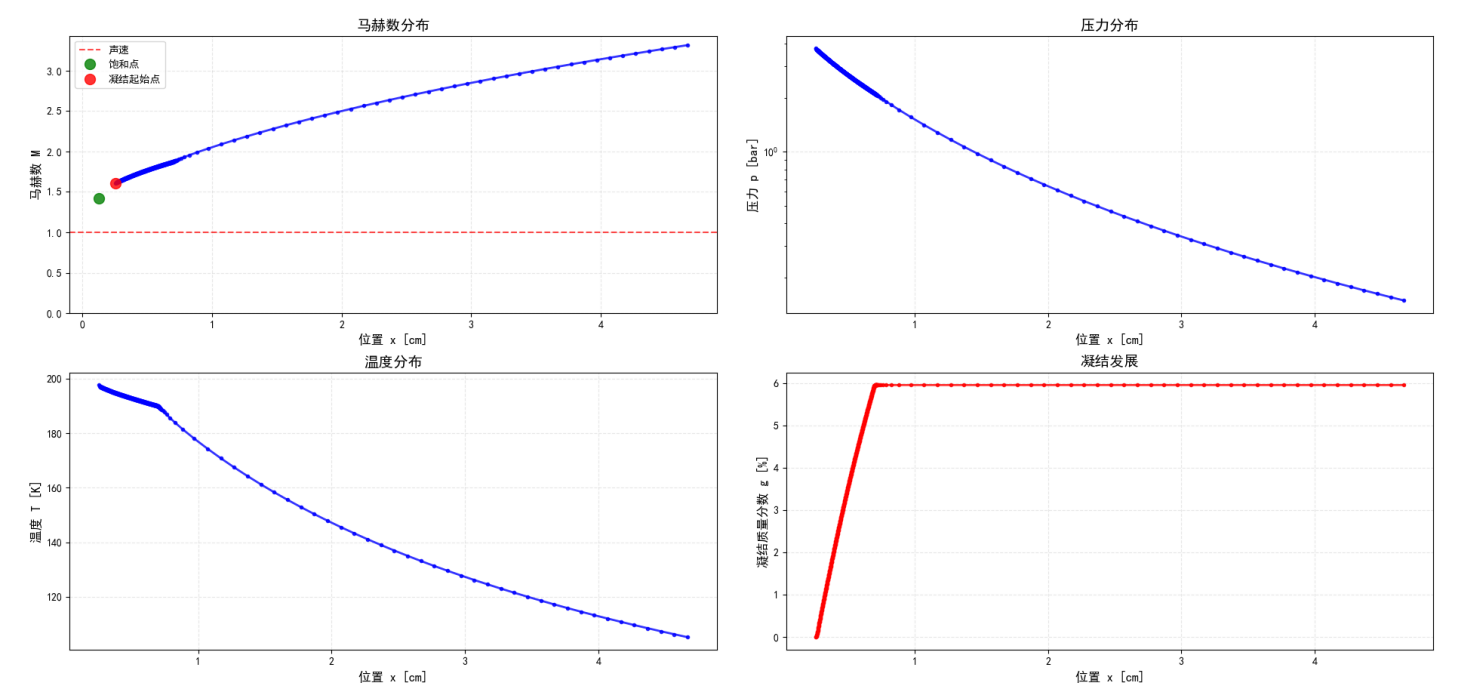
\includegraphics[width=0.8\textwidth]{figures/fig25.png}
		\caption{轴线温度、压力演化与凝结起始位置预测}
		\label{fig:phase_model1}
	\end{figure}
	\begin{figure}[H]
		\centering
		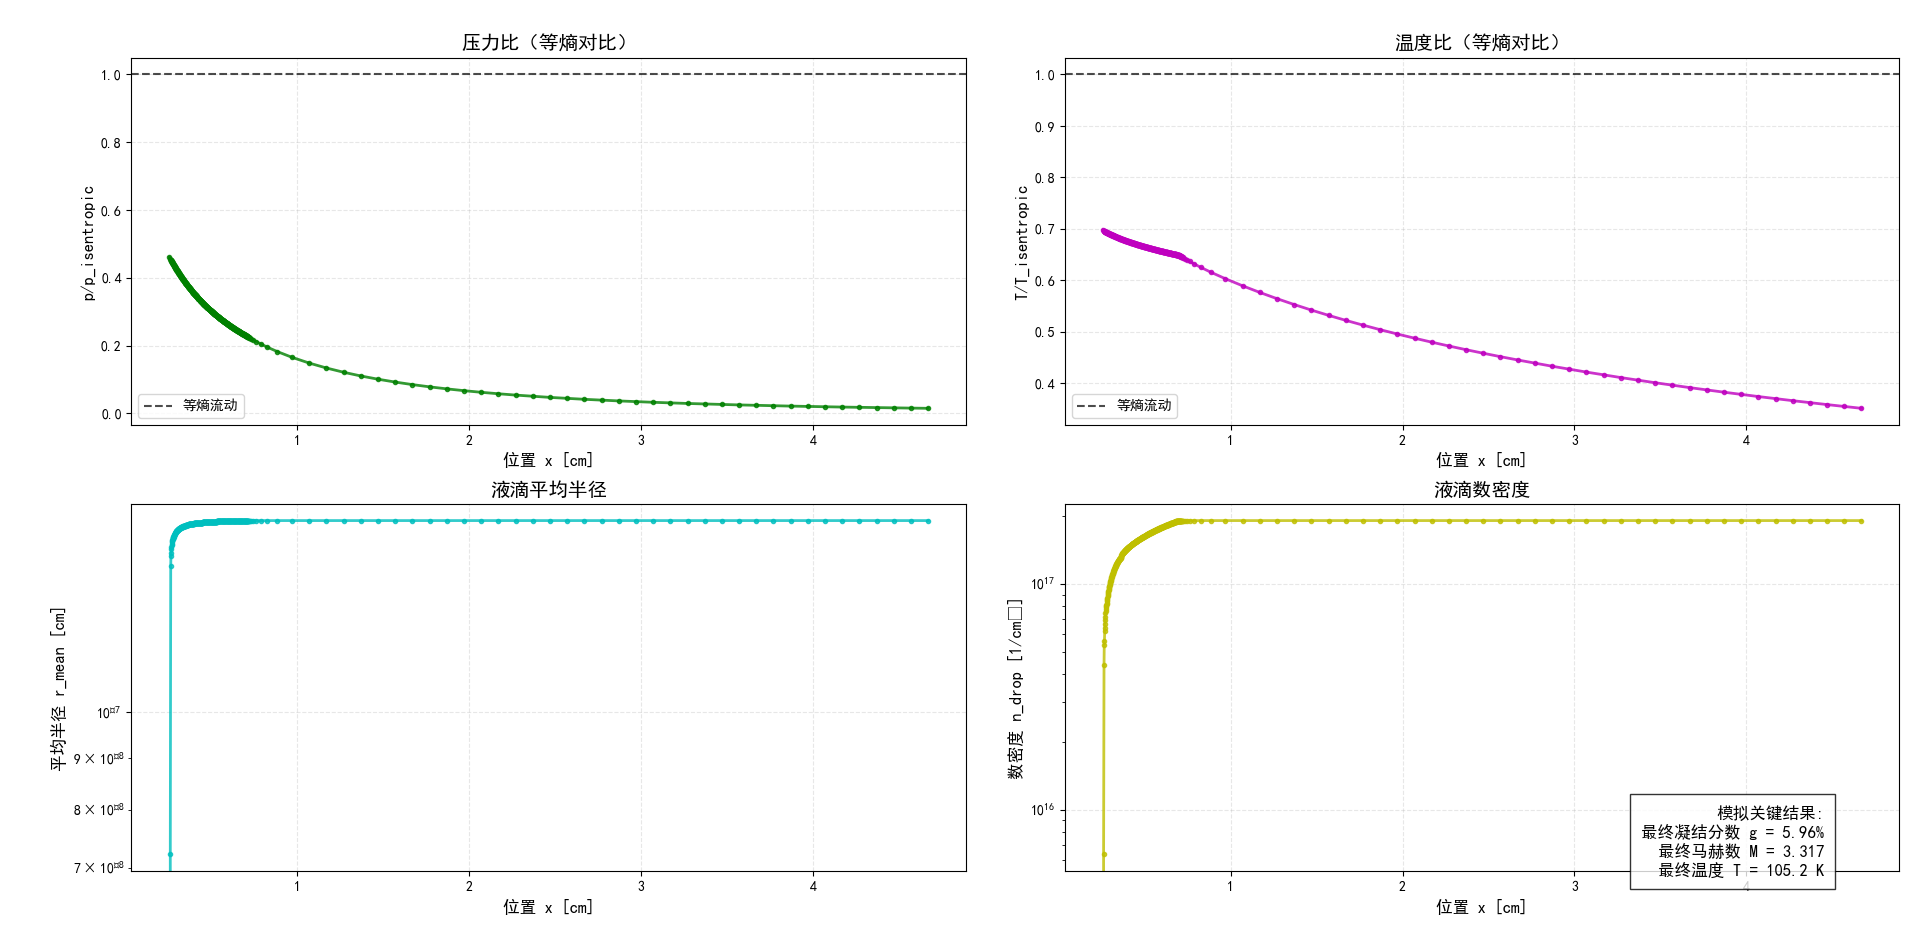
\includegraphics[width=0.8\textwidth]{figures/fig26.png}
		\caption{相变模型计算结果}
		\label{fig:phase_model2}
	\end{figure}
	计算结果表明：
	\begin{itemize}
		\item 等熵膨胀至$z\approx0.3$~mm处达到饱和点（$T\approx225$~K，$P\approx0.12$~MPa）；
		\item 过冷度达到5~K时（$z\approx0.8$~mm）触发成核，临界半径$r^*\approx1.2$~nm；
		\item 成核速率峰值$J\approx10^{20}$~m$^{-3}$s$^{-1}$出现在$z\approx1.5$~mm处；
		\item 马赫盘位置（$z\approx2.8$~mm）处温压骤升，成核速率下降三个数量级，已有团簇开始蒸发。
	\end{itemize}
	\subsubsection{与文献结果对比}
	将本模型预测的凝结起始位置（$z/D\approx0.8$）与Wu等（2021）的实验结果（$z/D\approx0.1-0.4$）对比，本文预测值偏下游。差异分析：
	\begin{itemize}
		\item 喷嘴几何差异：Wu等采用锥形扩张喷嘴，本文为直孔喷嘴，膨胀速率不同；
		\item 过冷度判定阈值：本文采用5~K，Wu等模型中可能更低；
		\item 后续需结合瑞利散射实验测量实际成核位置，校准模型参数。
	\end{itemize}
	模型预测的马赫盘后团簇蒸发趋势与文献一致，验证了模型的基本物理合理性。
	\subsection{本章小结}
	（1）温度反演综合不确定度约$\pm6$~K（95\%置信区间），主要来源于积分吸光度计算、探测噪声和光谱标定。后续应优先改进FSR标定精度和弱信号区域信噪比。
	（2）基于实验测量的流场温压数据，运行准一维相变模型预测凝结起始位置约$z=0.8$~mm（$z/D\approx0.8$），成核峰值位于$z\approx1.5$~mm。
	（3）与文献结果（$z/D\approx0.1-0.4$）存在差异，推测主要来源于喷嘴几何和过冷度判定阈值的不同。模型预测的马赫盘后团簇蒸发趋势与文献一致，验证了模型的基本物理合理性。后续需通过瑞利散射或团簇成像实验对模型进行校准，并在模型中逐步加入非定常项以改善小喉部面积工况下的收敛性。
	% ==================== 第七章 结论与展望 ====================

